\documentclass[border=0pt]{standalone}
\usepackage{pgfplots}
\pgfplotsset{width=\linewidth,compat=1.8}
\usepackage{pgfplotstable}
\usepackage{amsmath}
\begin{document}

\pgfplotsset{every tick label/.append style={font=\boldmath}}

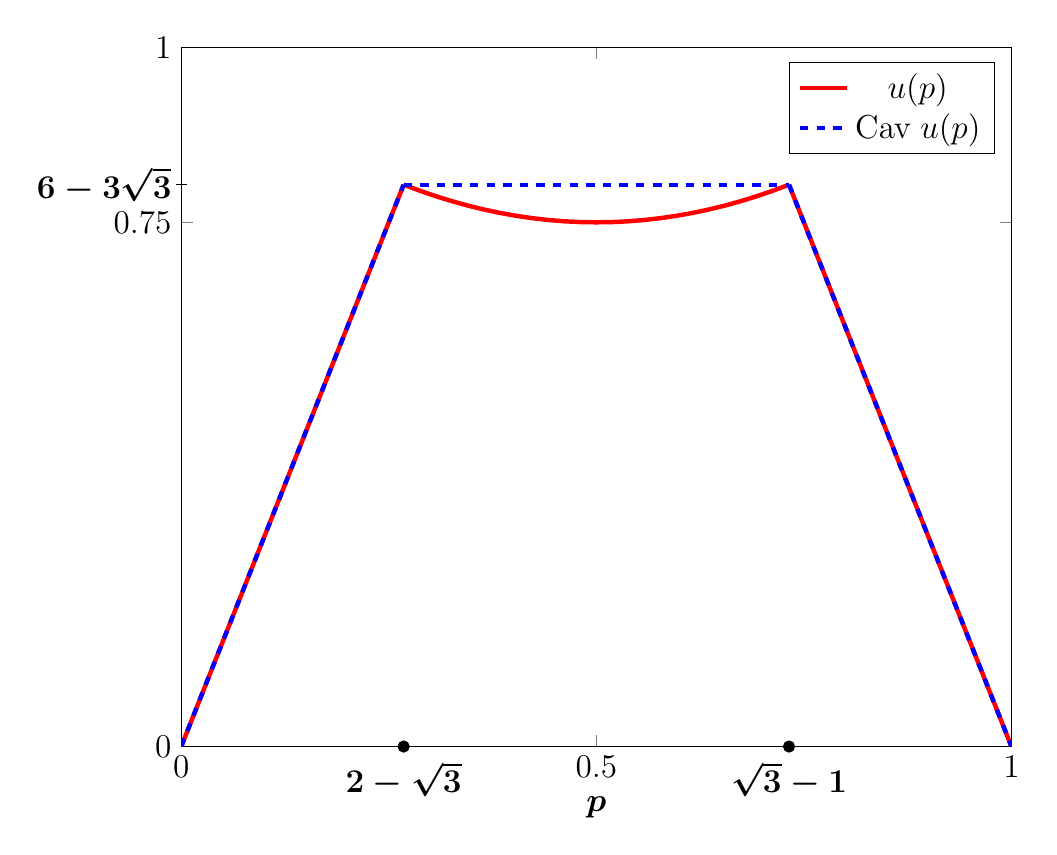
\begin{tikzpicture}
\tikzstyle{every node}=[font=\large]
\begin{axis}[ymax=1, ymin=0, xmin=0, xmax=1, xlabel= $\boldsymbol{p}$, xtick={0, 0.5, 1}, ytick={0, 0.75, 1},
    legend entries={$u(p)$, $\text{Cav}\;u(p)$},
        ]
    \addlegendimage{red, ultra thick}
    \addlegendimage{blue, ultra thick, dashed}
    \addplot[color=red, domain=0:0.2679, ultra thick]{3*x};
    \addplot[color=red, domain=0.2679:0.7321, ultra thick]{1-x*(1-x)};
    \addplot[color=red, domain=0.7321:1, ultra thick]{3*(1-x)};
    % cav
    \addplot[color=blue, dashed, domain=0:0.2679, ultra thick]{3*x};
    \addplot[color=blue, dashed, domain=0.2679:0.7321, ultra thick]{0.8038};
    \addplot[color=blue, dashed, domain=0.7321:1, ultra thick]{3*(1-x)};
    \addplot[
mark=*,only marks,
    nodes near coords={$\boldsymbol{2-\sqrt{3}}$},      % Label content
    nodes near coords align={south},     % Align label below the point
    every node near coord/.append style={anchor=north, yshift=-2pt} 
]
coordinates {(0.2679, 0)};
    \addplot[
mark=*,only marks,    
nodes near coords={$\boldsymbol{\sqrt{3}-1}$},      % Label content
    nodes near coords align={south},     % Align label below the point
    every node near coord/.append style={anchor=north, yshift=-2pt} 
]
coordinates {(0.7321, 0)};
    \addplot[
mark=-,only marks,    
nodes near coords={$\boldsymbol{6-3\sqrt{3}}$},      % Label content
    nodes near coords align={west},     % Align label below the point
    every node near coord/.append style={anchor=east} 
]
coordinates {(0, 0.8038)};
\end{axis}
\end{tikzpicture}
\end{document}